
\chapter{Algoritmos de detección y seguimiento de objetos}
\label{cha:algorithms}

\section{Introducción}
\label{sec:intro-algorithms}

\section{Algoritmos de detección de objetos}
\label{sec:tecnicas-utilizadas-detection}

\subsection{Fast R-CNN}
\label{subsec:fast-rcnn}

\subsection{Faster R-CNN}
\label{subsec:faster-rcnn}

\subsection{SSD: Single Shot MultiBox Detector}
\label{subsec:ssd}

\subsection{EfficientDet}
\label{subsec:efficientdet}

\subsection{YOLO: You Only Look Once}
\label{subsec:yolo}

Presentar YOLO y hacer énfasis en YOLOv4

\section{Algoritmos de seguimiento de objetos}
\label{sec:tecnicas-utilizadas-tracking}

\subsection{Filtro de Kalman}
\label{subsec:kalman-filter}

En azul y naranja las detecciones, deepsort cuadros delimitadores blancos.

Explicar filtro de Kalman

\textcolor{red}{Meter imágenes de ejemplo de se visualice bien el cuadro delimitador de detección y el de seguimiento}

\subsection{Algoritmo húngaro}
\label{subsec:hungarian-algorithm}

Explicar algoritmo húngaro.

\subsection{DeepSORT}
\label{subsec:deepsort}

Explicar que se trata de un algoritmo que combina El filtro de Kalman con el algoritmo húngaro.

\begin{figure}[ht]
\centering
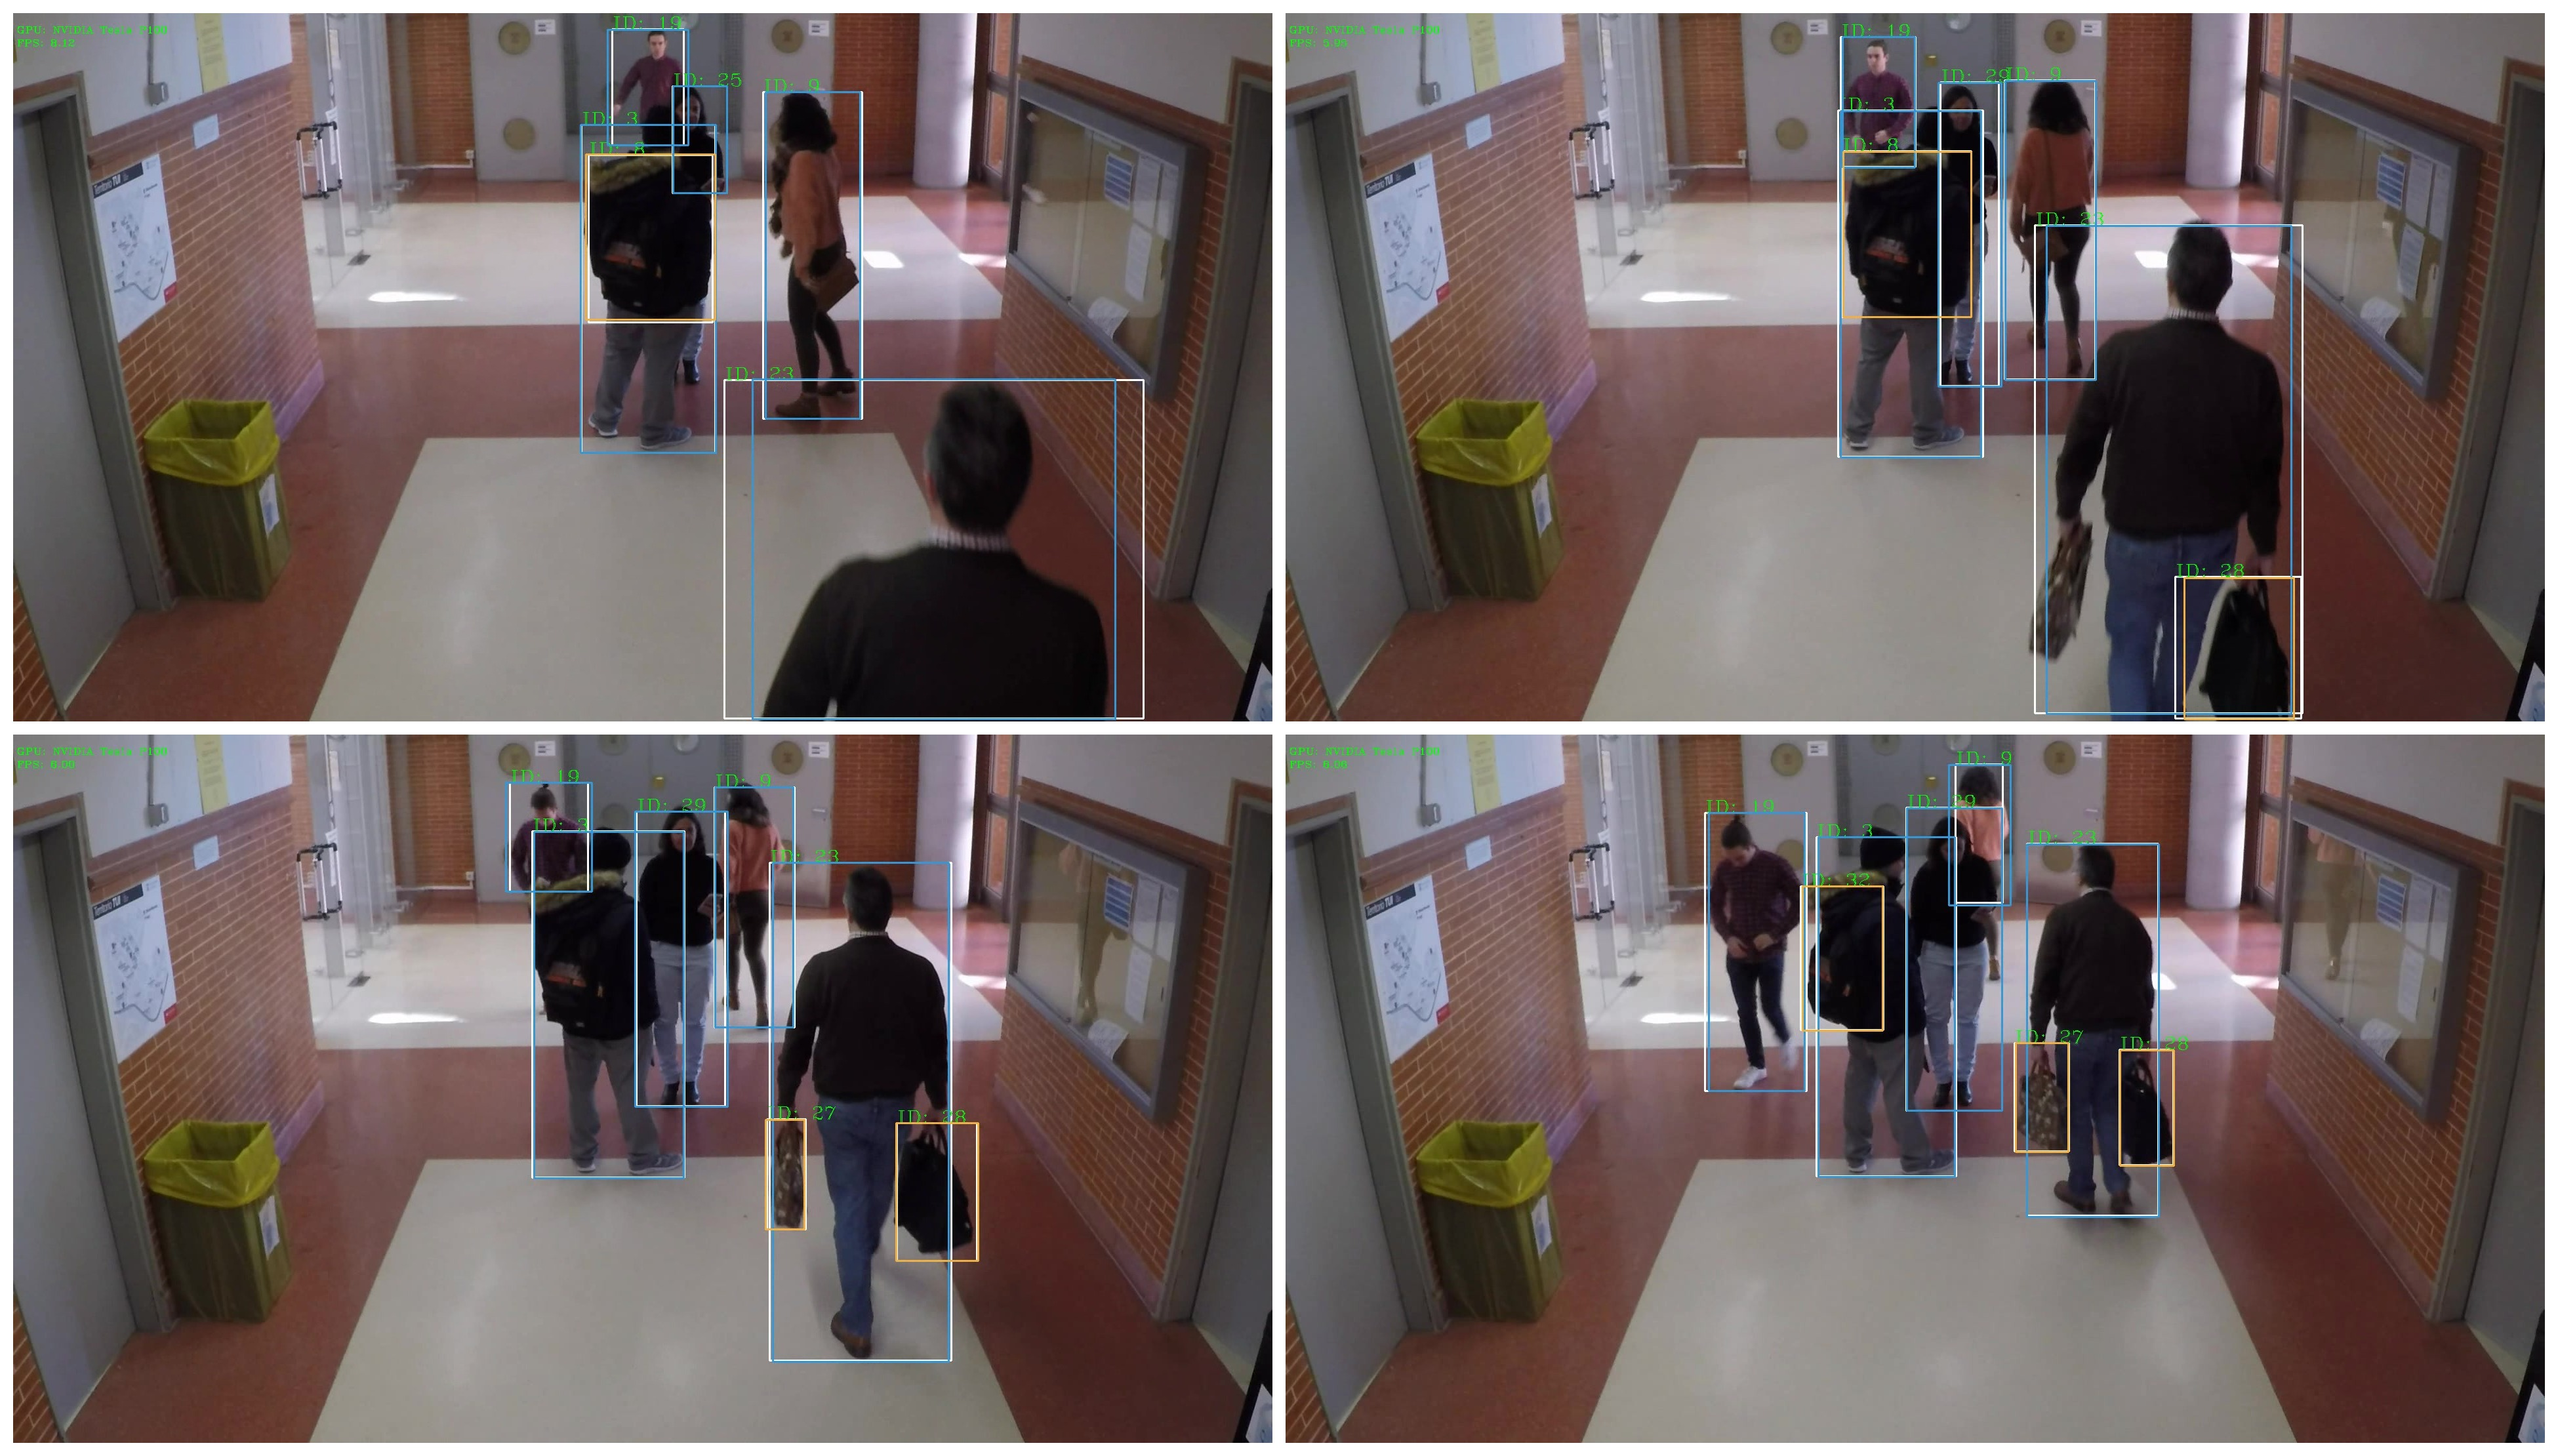
\includegraphics[width=1\textwidth]{img/chapters/algoritmos/deepsort-example.png}
\caption{\label{fig:tracking-example}Funcionamiento de Deepsort}
\end{figure}

\section{Conclusiones}
\label{sec:conclu-algoritmos}

\textcolor{red}{Aquí explicar con que detector de objetos el cual combinaré con DeepSORT para el desarrollo del algoritmo de detección de objetos abandonados.}
